\chapter{Projekcije podatkov}

Ena od težav, na katero naletimo pri uporabi hierarhičnega razvrščanja v skupine, je, da lahko napačno sugerira, da so si vsi predstavniki določene skupine med seboj podobni bolj, kot so podobni članom drugih skupin. Hierarhija skupin tako lahko daje uporabno in smiselno sliko podatkov, obenem pa je rigidna in ne dopušča "mehkega" članstva v skupinah.

Primer kaže slika~\ref{f-jeziki-hclust}. Angleščina je germanski jezik, ki se je razvijal pod vplivom romanskih, predvsem francoščine. Hierarhično gručenje jo mora nekam uvrstiti in dalo jo je k romanskim, čeprav bi jo pravzaprav lahko tudi k germanskim; če tega ne bi vedeli, bi iz gručenja sklepali, da je angleščina romanski jezik. Podobne težave ima italijanščina: je res podobnejša francoščini kot španščini? Morda ne. Postopek gručenja je najprej združil španščino in portugalščino; italijanščina je sicer morda blizu španščini, a tako različna od portugalščine, da je podobnost med italijanščino in francoščino večja kot med italijanščino in skupino španščina-portugalščina.

\begin{figure}[b!]
\begin{center}
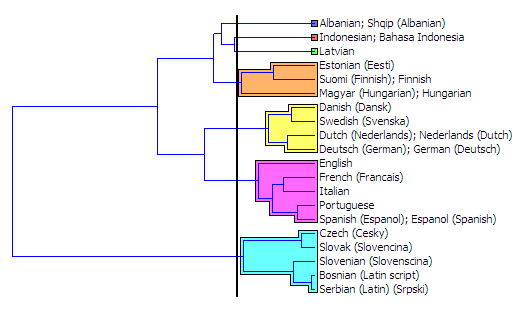
\includegraphics[width=12cm]{slike/jeziki-clustering.png}
\caption{Hierarhične gruče jezikov na podlagi podobnosti besed v prevodu Deklaracije o človekovih pravicah}
\label{f-jeziki-hclust}
\end{center}
\end{figure}

Razvrščanje v skupine je vseeno odličen postopek, ki ga bomo uporabili pač takrat, kadar želimo razvrstiti primere, na primer jezike, v skupine. Kadar pa si bolj želimo ustvariti podobo o podatkih, pa uporabimo katero od tehnik za projeciranje podatkov iz višjih v nižje -- recimo dvo- -- dimenzionalne prostore.

Med najbolj znanimi je večrazsežnostno lestvičenje ({\em multidimensional scaling}, MDS), ki iz matrike razdalj med objekti sestavi dvodimenzionalni zemljevid primerov, v katerih se razdalje čim bolj ujemajo z želenimi.

Nekoliko podobna tehnika je FreeViz. Za delovanje potrebuje seznam primerov v podobni obliki kot pri atributnem učenju: vsak primer je opisan z vrednostmi atributov in razredom. FreeViz poišče projekcijo v dve dimenziji, v katerih so primeri iz istega razreda čim bližje, primeri iz različnih razredov pa čim dalj eden od drugega.

Tretji postopek za projekcijo primerov v nižje-dimenzionalen prostor, ki ga bomo opisali, je analiza osnovnih komponent ({\em principle components analysis}, PCA). PCA je prav gotovo najbolj znana metoda za iskanje informativnih projekcij za množico podatkov. PCA  predpostavi, da se podatki, ki so sicer opisani z večjo množico atributov, v resnici nahajajo v nižjedimenzionalnem prostoru. PCA poišče osnovne komponente, to je, smeri, ki "napenjajo" množico primerov. Podobna metoda je faktorska analiza, obenem pa je PCA podoben tudi drugim oblikam dekompozicije, kot je, na primer, SVD. PCA se tipično ne uporablja za vizualizacijo podatkov, temveč predvsem za predstavitev podatkov z manjšo, razumljivejšo in zanesljivejšo množico atributov.

\section{Večrazsežnostno lestvičenje (MDS)}

Denimo, da trije Marsovčki ne bi prišli k Drejčku, temveč bi se z njim pogovarjali le po mobitelu. Radovedni Marsovčki bi radi izvedeli kaj o Sloveniji; ko bi jim Drejček tako našteval različne kraje in njihove znamenitosti, bi si Marsovčki počasi zaželeli malo več predstave o tem, kaj je kje. Drejček ima pri sebi zemljevid. Koordinatnega sistema še ne pozna, pač pa je ob zemljevidu tabela razdalj med vsemi pari (večjih) krajev. Je mogoče iz teh podatkov rekonstruirati zemljevid?

Seveda je. Drejček jim zrecitira tabelo in Marsovčkom je storiti naslednje: najprej vzamejo tri kraje, recimo Maribor, Kranj in Ljubljano, ter jih narišejo v trikotnik s podanimi razdaljami (v določenem merilu). Nato jemljejo vse ostale kraje, enega za drugim, in jih razpostavljajo na ustrezne razdalje od teh treh. Se lahko to kje zalomi? Prvo, kar bo šlo očitno vedno narobe, vendar nas sploh ne moti, je, da bo zemljevid obrnjen bogvekako, pa še prezrcaljen zna biti. Nič hudega, ne le Marsovčki, že Avstralci bi videli Slovenijo prezrcaljeno, če bi bila Zemlja steklena. Druga težava, do katere pri risanju Slovenije ne bo prišlo, pri risanju drugih reči pa, so nemogoče razdalje. Recimo, da bi Drejček Marsovčkom sporočil, da je od Ljubljane do Celja 65 kilometrov, od Celja do Maribora tudi 65, od Ljubljane do Maribora pa 150 km. V tem primeru, bodo rekli Marsovčki, si se, dragi Drejček, očitno zmotil: tega ni mogoče narisati, saj trikotnika s stranicami 65, 65 in 150 ni.

Idejo risanja zemljevidov iz podatkov lahko uporabimo tudi za podatke, ki v resnici niso prostorski. Tako lahko, recimo, narišemo zemljevid jezikov (Slika~\ref{f-jeziki-mds}), pri čemer so razdalje, tako kot pri gručenju, definirane na podlagi podobnih besed, ki se pojavljajo v prevodu Deklaracije o človekovih pravicah. Da bi bila slika preglednejša, smo na njej povezali 10\% najbolj podobnih parov jezikov. Slika lepo razpade na slovansko, romansko in germansko skupino, pri čemer je angleščina nekoliko na svojem (a še vedno bolj povezana z romanskimi kot germanskimi jeziki). Obenem je očitno tudi, da so si germanski in romanski jeziki med seboj podobni (zgodovinsko gledano je to najbrž posledica dejstva, da so se romanski jeziki razvijali iz latinščine pod vplivom prišlekov s severa), slovanski pa so nekje posebej.

\begin{figure}[tbp]
\begin{center}
\includegraphics[width=12cm]{slike/jeziki-mds.png}
\caption{Zemljevid jezikov, dobljen z večrazsežnostnim lestvičenjem; razdalje so definirane na podlagi besed v prevodu Deklaracije o človekovih pravicah}
\label{f-jeziki-mds}
\end{center}
\end{figure}


Prvega Drejčkovega problema tu ni: govoriti o tem, da je zemljevid jezikov obrnjen narobe, je nesmiselno, saj se jeziki v resnici ne nahajajo v prostoru. Pač pa imamo -- odvisno od tega, na kakšen način je definirana razdalja -- tu morda drugi problem: zemljevida, v katerem bi razdalje natančno odgovarjale želenim (v določenem merilu, seveda), morda sploh ni mogoče narisati, saj takšna postavitev ne obstaja. Nič ne de: namesto ``točnega'' zemljevida, bomo zadovoljni tudi s približnim. 

Kako ga narisati? Takole: objekte si predstavljajmo kot kroglice, ki jih povežemo z vzmetmi, katerih dolžine ustrezajo želenim razdaljam (predstavljajmo si, da gre za posebne vzmeti, ki se ne zavozljajo temveč lahko prehajajo ena skozi drugo). Dobimo veliko žogo iz krogel in vzmeti, a ko jo izpustimo fizika opravi svoje -- krogle se razletijo in razmestijo tako, da so vse vzmeti karseda ``sproščene'', ne predolge in ne prekratke.

Računalniško izvedbo tega algoritma imenujemo večrazsežnostno lestvičenje ({\em multidimensional scaling}, MDS). Formalno ga zastavimo tako, da definiramo energijo sistema ali napetost ({\em stress}) kot, recimo,
$$\sigma(\mathbf{X}) = \sum_{i\ne j} (d_{ij} - \delta_{ij})^2,$$
kjer je $\mathbf{X}$ trenutni razpored točk, $d_{ij}$ in $\delta_{ij}$ pa trenutna in želena razdalja med točkama $i$ in $j$. Večrazsežnostno lestvičenje poišče razpored $\mathbf{X}$ z najmanjšo napetostjo $\sigma(\mathbf{X})$.

Kako minimizirati takšno funkcijo? Analitično ne bo šlo. Za to bi bilo potrebno odvesti $\sigma(\mathbf{X})$ po vseh koordinatah ($x_i$ in $y_i$) in poiskati ničle. Razdalja med točkama $i$ in $j$ je enaka $d_{ij}=\sqrt{(x_i-x_j)^2+(y_i-y_j)^2}$, torej bo
\begin{eqnarray*}\frac{\partial\sigma({\mathbf{X}})}{\partial x_i} & = &
\sum_{j\ne i} \frac{\partial\sigma({\mathbf{X}})}{\partial d_{ij}}\frac{d_{ij}}{\partial x_i} \\ & =
& \sum_{j\ne i} -2\left(\delta_{ij}-\sqrt{(x_i-x_j)^2+(y_i-y_j)^2}\right) \frac{(x_i-x_j)}{\sqrt{(x_i-x_j)^2+(y_i-y_j)^2}}
\end{eqnarray*}
Pri stotih točkah bi dobili sistem z dvesto takšnimi enačbami; ideji o direktnem napadu se torej raje odpovemo.

Drug, izvedljiv postopek je gradientna metoda: izračunamo gradient funkcije $\sigma(\mathbf{X})$, se pravi odvod po vseh spremenljivkah. To smo pravzaprav storili že zgoraj. Izberemo si poljuben začetni razpored točk, vstavimo koordinate v odvode, dobimo gradient (vektor odvodov) in se pomaknemo v smeri nasprotni gradientu, se pravi, vse točke pomaknemo v smer, kamor jih potiskajo odvodi. Kot vemo iz analize ali od kod drugod, nas bo to počasi pripeljalo v minimum. (Takšen algoritem počne natančno to, kar bi počela narava z vzmetmi: odvod energije po položaju je sila, torej gradientna metoda pomika vse točke v smeri sile.)

Gradientna metoda bi delovala, vendar ne prav dobro. Bila bi počasna in velikokrat bi nas (lahko) pripeljala le v lokalni minimum. V fizikalni metafori, krogle in vzmeti bi se znašle v neki lokalno stabilni konfiguraciji, vendar bi jih bilo mogoče ``potisniti'', preobrniti tako, da bi se ``zoptimizirale'' tudi v kaj boljšega.

V svetu optimizacijskih problemov je gradientna metoda le metoda grobe sile, ki jo bomo uporabili, če se ne moremo spomniti ničesar boljšega. Eden od boljših postopkov je ``majorizacija''. Označimo funkcijo, katere minimum iščemo, z $f(x)$. Recimo, da si znamo izmisliti, neko drugo funkcijo $g(x, y)$, ki je stalno večja ali enaka $f(x)$ (torej, za vsak $y$ velja $g(x, y)\ge f(x)$ pri vsakem $x$), v točki $g(x, x)$ pa velja $g(x, x)=f(x)$. Funkcija $g(x, y)$ naj bo takšna, da znamo dobro poiskati vrednost $x$, pri katere doseže minimum. Zdaj lahko počnemo tole: izmislimo si začetni $x_0$. Pri njem, vemo, velja $g(x_0, x_0)=f(x_0)$. Minimiziramo funkcijo $g$ in dobimo nov, boljši $x$ - označimo ga z $x_1$. Vrednost $g(x_1, x_0)$ je manjša ali enaka vrednosti $g(x_0, x_0)$, saj smo minimizirali $g$ po prvem argumentu. Po drugi strani, spet po definiciji funkcije $g$, velja $f(x_1) \le g(x_1, x_0)$. Imamo torej
$$f(x_1) \le g(x_1, x_0) \le g(x_0, x_0) = f(x_0)$$
Postopek ponovimo z $x_1$, da pridelamo naslednji, še boljši $x_2$.

Takšna optimizacija je, tako kot gradientna metoda še vedno iterativna, vendar hitrejša. Koliko hitrejša, je odvisno od tega, kako dobro $g(x, y)$ smo poiskali; $g(x, y)$ se mora čim tesneje prilegati $f(x)$, poleg tega pa jo moramo biti zmožni čim boljše optimizirati.

Algoritem večdimenzionalnega lestvičenja, ki deluje na ta način, se imenuje SMACOF ({\em Scaling by majorizing a complicated function}). SMACOF je hitrejši od gradientne metode, dela večje korake in se manjkrat zatakne v lokalnih ekstremih, zato je uporabnejši za (realistične) primere, v katerih je točk veliko.

Za izračun napetosti lahko namesto gornje, naivne formule uporabljamo tudi takšne, ki uteži prispevke parov (predpišemo lahko, za katere pare si še posebej želimo, da bi razdalja ustrezala pravi), poleg tega pa lahko napetost posameznega para normiramo tako, da jo delimo z želeno ali s trenutno razdaljo.

Slika~\ref{f-zoo-mds} kaže zemljevid živali. Razdalje med pari živali so izračunane kot evklidske razdalje med atributi, ki jih opisujejo. Točke, ki predstavljajo živali, smo obarvali glede na vrsto -- vijolični so sesalci, rdeče ptice, oranžno žuželke. Povezani so pari živali, ki so si med seboj najbolj podobne.

\begin{figure}[tbp]
\begin{center}
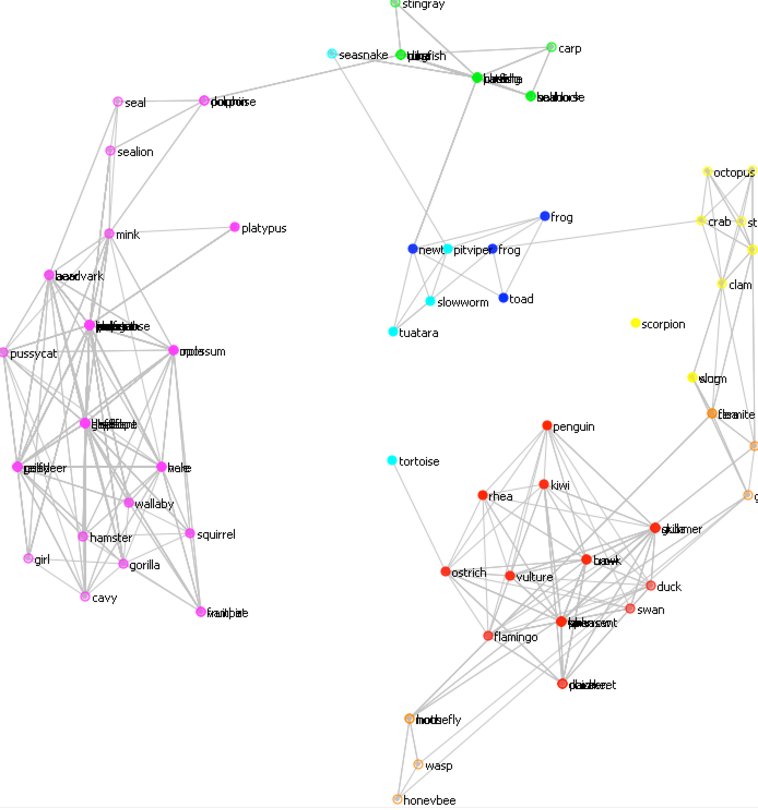
\includegraphics{slike/zoo-mds.pdf}
\caption{Zemljevid živali (podatkovna zbirka Zoo)}
\label{f-zoo-mds}
\end{center}
\end{figure}

Čeprav MDS ni uporabljal podatkov o vrstah živali, so različne vrste na zemljevidu dobro ločene. Vidimo tudi nekaj podobnosti med živalmi: morske sesalce je MDS postavil v bližino rib; dvoživke so blizu rib in nevretenčarjev, predvsem morskih; žuželke so pomešane s ptiči.

Vidimo tudi težavo: žuželke so razdeljene v dve skupini. MDS se je očitno znašel v lokalnem ekstremu, saj bi morale ose in čebele k ostalim žuželkam, vendar bi jih moral optimizacijski postopek peljati okrog ptičev. To se zgodi kar pogosto in pomagamo si tako, da podatke nekoliko potresemo, naključno premaknemo točke, ali pa začnemo celotno optimizacijo znova.

Večrazežnostno lestvičenje je torej postopek, ki vizualizira podatke v obliki zemljevida. Podatki so opisani s seznamom primerov in razdalj med njimi; lastnosti primerov niso potrebne in jih ne znamo upoštevati (razen, če iz le-teh računamo razdalje, kot smo storili pri živalih). Zemljevid je nezanesljiv v tem smislu, da bodo različne naključne začetne postavitve vodile v različne končne slike, a vsaka od njih nam lahko nudi drugačen pogled na podatke. Prav tako je nezanesljiv položaj posameznih točk; dogaja se, da je točka obtičala v lokalnem minimumu, čeprav v resnici ne sodi na to mesto. Takšne točke lahko prepoznamo, če zemljevidu dodamo povezave med najbolj podobnimi pari. Obenem nam takšne povezave pomagajo brati sliko. MDS ne sestavlja gruč, pač pa lahko gruče razberemo sami.


\section{FreeViz}

Denimo, da imamo primere, ki so opisani z atributi, za vsak primer pa je podan tudi razred. Zemljevid takšnih podatkov bi sicer lahko narisali z večrazežnostnim lestvičenjem, kot smo to storili pri živalih, vendar bi tako zanemarili podatke o pripadnosti razredom. Poleg tega si pri takšnih podatkih navadno želimo imeti model, s katerim bomo lahko uvrščali nove podatke; MDS nam tega ne omogoča.

Želimo si torej metodo, ki vsaki točki priredi njeno mesto na podlagi vrednosti njenih atributov, pri čemer naj bo mesto določeno tako, da bodo primeri iz istega razreda blizu eden drugemu.

Primer takšne metode je FreeViz. FreeViz je linearna projekcija. Če imajo primeri $k$ atributov, bomo rekli, da se nahajajo v $k$-dimenzionalnem prostoru; vsak primer je točka in njene koordinate so pač vrednosti atributov. Primere bomo pisali z vektorjem-vrstico $\mathbf{e} = [e^1, e^2, 
\ldots, e^k]$. Vsakemu atributu ustreza ena dimenzija, en bazni vektor. Linearne projekcije so določene s slikami baznih vektorjev. Naj bodo torej $\mathbf{a^0}, \mathbf{a}^1, \ldots, \mathbf{a}^k$ slike baznih vektorjev, $\mathbf{a^i} = [a_x^i, a_y^i]$. Zberimo jih v matriko, $\mathbf{A} = [\mathbf{a^0}, \mathbf{a}^1, \ldots, \mathbf{a}^k]^T$. Projekcija primera $\mathbf{e}$ je tako enaka $\mathbf{e'} = \mathbf{eA}$ (ker so naši vektorji vrstice in ne stolpci, moramo množiti z leve, ne z desne). Naloga projekcije je poiskati dobro matriko $\mathbf{A}$.

Kaj pomeni dobro matriko? Določiti moramo funkcijo, ki jo želimo optimizirati. Za razliko od MDSa tokrat ne bomo definirali energije, temveč silo (torej v resnici ne definiramo funkcije, ki jo želimo optimizirati, temveč njen gradient). Točki, ki ustrezata primeroma iz istega razreda, se bosta privlačili, točke, ki ustrezajo primerom iz različnih razredov, se bodo odbijale. Za razliko od tega, česar smo navajeni iz fizike, bodo privlačne sile naraščale z razdaljo. To je smiselno zato, ker je točke, ki so izgubljene nekje daleč od svojih, težko privleči mimo vseh točk, ki so jim na poti, zato jih bomo vlekli z veliko silo. Po drugi strani pa dveh točk iz istega razreda, ki so že prišle blizu ena drugi, nima smisla tlačiti še bližje. Z odbojnimi silami je ravno nasprotno: točke različnih razredov, ki so si blizu skupaj želimo na vsak način spraviti narazen. Točk različnih razredov, ki so že daleč narazen, pa nima smisla še bolj odbijati. Zato bodo odbojne sile z razdaljo padale.

Naj bo torej $\mathbf{F_{ef}}$ sila, s katero točka $f$ deluje na točko $e$; definiramo jo lahko recimo, tako, da za točke istega razreda narašča in za točke različnih razredov pada kar linearno z razdaljo (po želji pa lahko izberemo tudi kvadrat ali kako drugo primerno funkcijo razdalje). Naj bo $\mathbf{F_e} = \sum_{f\ne e} \mathbf{F_{ef}}$ vsota vseh sil na točko $i$. Iz tega lahko izračunamo, kakšna sprememba projekcije $\mathbf{A}$ zmanjša energijo sistema:
$$\frac{\partial E}{\partial a^i_x} = -\sum_e F_{e, x}e^i,$$ pri čemer je $F_{e, x}$ komponenta $x$ sile $\mathbf{F_e}$; enačba za smer $y$ je ekvivalentna. Vsako od projekcij baznih vektorjev pomaknemo v tej smeri in to ponavljamo, dokler se optimizacija ne ustavi v (lokalnem) minimumu.

Fizikalno si lahko predstavljamo, da so točke delci, ki se odbijajo oziroma privlačijo med seboj, obenem pa so ti delci pripeti na osi, ki predstavljajo atribute. Sile na delce se tako prenašajo na atribute. Kako močna je vez med delci in atributi, je odvisno od vrednosti atributa ($e^i$). 

\begin{figure}[tbp]
\begin{center}
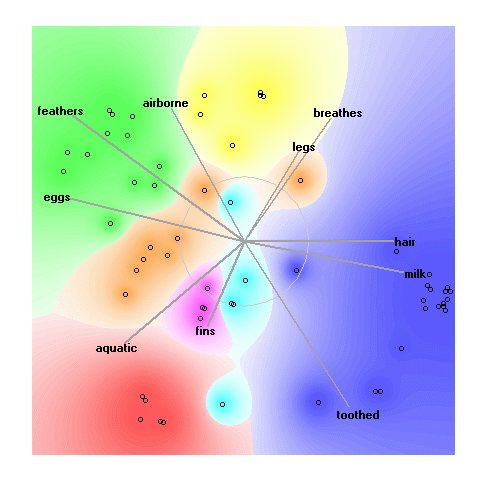
\includegraphics[width=12cm]{slike/zoo-freeviz.png}

\includegraphics[width=12cm]{slike/zoo-legenda.png}
\caption{Projekcija FreeViz iz podatkov o živalih}
\label{f-zoo-freeviz}
\end{center}
\end{figure}


Rezultat takšne projekcije na podatkih o živalih vidimo na sliki~\ref{f-zoo-freeviz}. Iz nje lahko, če znamo, razberemo veliko lastnosti podatkov.

Različna področja so obarvana glede na prevladujočo živalsko vrsto - sesalci so modri, ribe rdeče in tako naprej. Osi ustrezajo atributom; smer osi nakazuje regijo, živalsko vrsto, ki jo sugerira visoka vrednost tega atributa. Vsi atributi, razen števila nog, so binarni, torej v tem primeru recimo dlake in zobje kažejo, da je žival verjetno sesalec. Iz osi torej razberemo povezavo med atributi in razredi, vidimo, katera živalska vrsta je značilna za posamezno lastnost, oziroma, katere lastnosti so značilne za posamezno živalsko vrsto.

FreeViz lahko beremo -- podobno kot MDS -- kot zemljevid. Ptiči in žuželke so si med seboj podobne; oboji letijo, zato v njuno smer kaže atribut {\em airborne}. Prav tako so si podobne ribe in dvoživke.

Vidimo lahko tudi podobnosti med atributi: kosmate živali dajejo mleko; živali, ki letajo, imajo perje, živali, ki plavajo, plavuti in živali, ki dihajo, noge. Obenem razberemo tudi glavne osi, po katerih lahko ločimo živali: žival bodisi daje mleko, bodisi vali jajca (vodoravna os) in je vodna žival s plavutmi ali pa dihajoča žival z nogami.

Osi, ki predstavljajo atribute, so različno dolge; čim pomembnejši je atribut, tem daljša je pripadajoča os. Manj pomembni atributi, katerih osi bi bile krajše od kroga v sredini, zaradi preglednosti niso narisani.

Končno, FreeViz je mogoče uporabljati tudi za uvrščanje primerov. Nov primer, katerega vrednosti atributov poznamo, razreda pa ne, lahko projeciramo in preverimo, v katero regijo je padel. Če v modro, je najbrž sesalec, če v zeleno, ptič\ldots

Ob uporabi FreeViza se moramo zavedati, da gre le za projekcijo v dvodimenzionalni prostor. Vse, kar vidimo, ni nujno resnično. Določeni atributi so morda tam, kjer so, samo zato, ker nekje pač morajo biti. Če uporabljamo FreeViz za iskanje vzorcev, moramo z njim dobljene vzorce preveriti, po možnosti na povsem novih podatkih ali pa jih primerjati z ekspertnim predznanjem o problemu.

FreeViza ne smemo uporabiti, kadar je število atributov primerljivo številu primerov ali celo večje. V tem primeru je mogoče kar analitično poiskati neskočno število rešitev, pri katerih so vse sile enake 0, razpored točk pa je v tem primeru nesmiseln.

Slabost FreeViza je tudi, da v osnovi temelji na gradientni metodi in postane pri velikem številu točk počasen. Na lokalne ekstreme pa je, kakor je videti, dokaj neobčutljiv.

\section{Analiza osnovnih komponent}

Analiza osnovnih komponent (angl. {\em principal component analysis}) je tehnika, ki večdimenzionalne podatke preslika v nižjedimenzionalni prostor tako, da je varianca proiciranih podatkov največja. Opišimo ta problem in njegovo rešitev intuitivno, nato pa z nekaj matematike poiščimo njegovo analitično rešitev.

\subsection{Kaj so sploh glavne komponente?}

Tehika PCA pokriva prostor med MDS in FreeViz-om: imejmo množico primerov, ki so opisani z atributi, vendar niso razdeljeni v razrede. Množica atributov je velika in slutimo, da so med seboj korelirani. Tipičen primer so testi inteligentnosti: denimo, da je tisoč ljudi reševalo test, ki vsebuje sto problemov in vsaka rešitev je ocenjena z numerično oceno, recimo med 0 in 10. Potencialni delodajalci se zanimajo za inteligentnost teh in prihodnjih reševalcev testa.

Inteligentnost bi lahko izrazili z eno samo številko, ki bi predstavljala poprečni rezultat prek vseh stotih nalog. Tako se, v grobem, računa inteligenčni količnik. Delodajalcem to ne bi zadoščalo: naloge merijo inteligenco v več pogledih, nekatere so bolj matematične narave, druge jezikovne in tretje testirajo prostorsko predstavo, večina nalog pa morda zahteva različne kombinacije teh sposobnosti. Po drugi strani delodajalci tudi ne bi bili preveč zadovoljni, če rezultate sporočimo kot seznam točk, ki jih je reševalec dobil pri vsaki od stotih nalog. Inteligenco si želimo izraziti z nekaj, recimo sedmimi, številkami, ki bodo izražale testirančeve zmožnosti v sedmih različnih pogledih.

To, kar iščemo v tem primeru, je metoda, ki poišče linearno preslikavo iz stodimenzionalnega prostora vprašanj v nekajdimenzionalni prostor odgovorov. (Čemu linearno? Ker je najpreprostejša. Za (zanesljivo) sestavljanje nelinearne preslikave namreč potrebujemo veliko več podatkov kot za linearno, zato se nelinearnim preslikavam izogibamo, če zanje ni res dobrega razloga.)

Metod, ki to znajo, je kar nekaj. Za primere, kot je gornji, se najpogosteje uporablja faktorska analiza ({\em factor analysis}). Ta predpostavlja, da so spremenljivke, ki jih merimo (uspešnost reševanja nalog) linearna kombinacija vrednosti spremenljivk, ki jih ne moremo neposredno izmeriti in jih imenujemo latentne spremenljivke ({\em latent variables}). Faktorska dekompozicija odkrije povezavo med merjenimi in latentnimi spremenljivkami.

Nekoliko preprostejša metoda je analiza osnovnih komponent ({\em principal component analysis}, PCA). Ta išče smeri, osnovne ali glavne komponente, ki pojasnijo čim več variance v podatkih.

Za primer vzemimo enega od omenjenih Marsovčkov, ki gre na sprehod po vesolju. Daleč od vseh planetov in vesoljskih ladij naleti na roj vesoljskih muh, ki negibno lebdijo v vesolju. Vzame svoj hologramski fotoaparat in jih fotografira. Ko se vrne na Mars, namerava poročati Drejčku, ki se je medtem naučil uporabljati koordinatni sistem, o svoji najdbi in mu pove koordinate muh na svoji sliki, zato si na sliki že označi koordinatni sistem (Slika~\ref{f-muhe}, koordinatne osi v levem spodnjem kotu). 

\begin{figure}[tbp]
\begin{center}
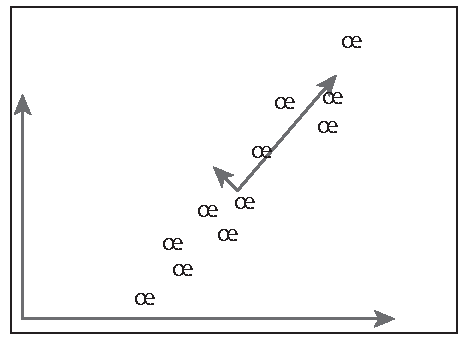
\includegraphics[width=7cm]{slike/muhe.pdf}
\caption{Slika vesoljskih muh s koordinatnim sistemom v levem spodnjem kotu slike in z osnovnima komponentama}
\label{f-muhe}
\end{center}
\end{figure}

A še preden telefonira Drejčku, opazi, da so muhe razporejene skoraj v ravni črti, ki gre v diagonalni smeri prek slike. Predpostavi, da so muhe pravzaprav hotele lebdeti v ravni črti in so vsi odmiki od te črte le naključna odstopanja. Drejčku bo zato opisal položaje muh le vzdolž te osi. Namesto s tremi koordinatami bo tako sporočil koordinate muh le z eno samo (če Drejčka zanima, kako je videti fotografija, pa mu sporoči še enačbo premice).

Drejček torej izve koordinate muh, vendar mu radovednost ne da miru in hoče izvedeti njihov položaj točneje. Kot je znano, delajo hologramski fotoaparati tridimenzionalne slike, vendar Marsovček ugotovi, da so muhe praktično v isti ravnini, zato mu sporoči, kot drugo koordinato, le odstopanja muh v smeri druge glavne komponente, ki smo jo označili na sliki. Ta komponenta je manj pomembna, zato je narisana krajše. Ker Drejček še vedno ni zadovoljen in je prepričan, da muhe ne lebdijo v ravnini, temveč so malo razmetane tudi v tretji smeri, mu Marsovček končno pove še tretjo, najmanj pomembno koordinato. Opis položajev muh je s tem točen.

Analiza osnovnih komponent je postopek, ki za podane koordinate točk poišče glavne komponente, torej smeri, v katerih se raztezajo podatki. Komponente so urejene po pomembnosti; v statističnem jeziku bi rekli, da prva pojasni največ variance (točke so najbolj raztegnjene v tej smeri), druga pojasni čimveč preostale variance in tako naprej. Če pogledamo s perspektive atributov ali, kot bi rekli statistiki, spremenljivk, analiza osnovnih komponent zamenja originalne spremenljivke z novimi, ki so sestavljene kot linearna kombinacija izvirnih.

Geometrijsko gledano PCA zamenja izvirni koordinatni sistem, katerega osi ustrezajo izvirnim spremenljivkam, z novim, katerega osi kažejo v smereh največje razpršenosti podatkov. Če se spomnimo, da v vesolju ni tal, bi lahko rekli, da je Marsovček obrnil fotoaparat, kakor je želel in s tem si je izbral nek koordinatni sistem, ki pa ni v nobenem primeru "posvečen", boljši od drugih koordinatnih sistemov. Koordinatni sistem, ki ga poišče PCA, pa je posvečen v tem smislu, da so osi izbrane glede na padajočo varianco -- prva os je pobere največ, kolikor se da, druga pobere največ preostale variance in tako naprej.

Če uporabimo toliko osnovnih komponent, kolikor dimenzij imajo začetni podatki, so vse točke točno opisane, le koordinatni sistem je drugačen (za primer se spomnimo na muhe). Navadno pa jih vzamemo manj: ko je pojasnjene, recimo 95\% variance, nam to zadošča.

Spomnimo se spet naloge z inteligenco in privzemimo, da smo naredili analizo osnovnih komponent in odkrili, da skoraj vso varianco pojasnimo z -- da bo lažje razmišljati -- samo dvema izpeljanima spremenljivkama. Spremenljivki sta opisani kot linearna kombinacija osnovnih stotih. Če pogledamo tidve kombinaciji, odkrijemo, recimo, da je prva komponenta enaka 0,6-krat vsota točk pri prvih štiridesetih vprašanjih in 0,3-krat vsota točk pri vprašanjih 41-60. Druga komponenta je enaka 0,4-krat vsota točk pri vprašanjih 41-50 in 0,7-krat vsota točk pri vprašanjih 71-100. Zdaj se poglobimo v vprašanja in odkrijemo, da je prvih štirideset vprašanj s področja matematike, pa tudi naslednjih dvajset (41-60) je povezanih z matematiko, čeprav manj. Za vprašanja 41-50 in 71-100 vidimo, da so povezana z jezikovnimi sposobnostmi. Na vprašanja 61-70, ki se ne pojavijo v nobeni od teh dveh komponent, so vsi ljudje odgovarjali skoraj enako, zato je, z drugimi besedami, varianca tam takoj majhna, da ni česa pojasnjevati.

Zdaj lahko uporabimo komponenti kot koordinatni osi; za vsakega testiranca izračunamo vrednost prve in druge spremenljivke ter narišemo točko na pripadajoče koordinate. Tako smo dobili razpored ljudi v dvodimenzionalno definirani inteligenci: tisti na desni so dobri matematiki, tisti zgoraj jezikoslovci; zgoraj desno so ljudje, ki so dobri obojem, spodaj levo tisti, ki v ničemer.

V resnici bi inteligenca razpadla na kakih sedem komponent, a ideja je podobna: analiza osnovnih komponent združi atribute v smiselne skupine in pove, koliko je posamezni izvirni atribut zastopan v posamezni skupini. Če imamo srečo, je mogoče skupinam -- izpeljanim spremenljivkam -- z opazovanjem njihove sestave določiti pomen. Mimogrede vidimo tudi, katere osnovne spremenljivke so nepomembne.

Nove, izpeljane spremenljivke, so boljše od starih, saj jih je manj (ob čemer je izguba informacije majhna, saj smo jih sestavljali s tem v mislih) in so bolj stabilne, saj so sestavljene iz več osnovnih atributov. Tako je imel testiranec morda smolo pri eni matematični nalogi, vendar glavna komponenta računa uteženo poprečje prek vseh matematičnih nalog.

Analizo osnovnih komponent lahko uporabimo kot tudi vizualizacijski pripomoček, navadno tako, da rišemo točke v projekciji, ki jo določata prvi osnovni komponenti.

Pomanjkljivost analize osnovnih komponent je, da ne upošteva razreda. V problemu, kot smo ga zastavili -- imamo podatke, ki niso razvrščeni v razrede -- nas to ne moti. Včasih pa bi radi z analizo osnovnih komponent poiskali primerne atribute za razvrščanje. Vesoljske muhe se, kot ve vsak, ki ima za sabo Osnove eksobiologije 1, delijo na muhe kratnice in muhe deljnice. Denimo, da so na fotografiji, ki jo je naredil Marsovček, lebdele, kot kaže Slika~\ref{f-muhe-nadzorovane}, nam prva komponenta o vrsti muhe ne pove ničesar, druga pa vse. V tem primeru lahko uporabimo nadzorovano analizo osnovnih komponent ({\em supervised principal component analysis}), o kateri pa se pri tem predmetu ne bomo učili.


\begin{figure}[tbp]
\begin{center}
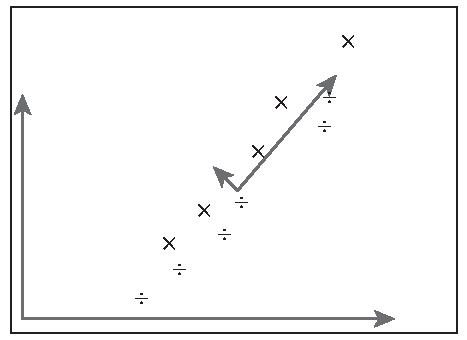
\includegraphics[width=7cm]{slike/muhe-nadzorovane.pdf}
\caption{Slika vesoljskih muh kratnic in deljnic}
\label{f-muhe-nadzorovane}
\end{center}
\end{figure}


\subsection{Računanje glavnih komponent}

Izkaže se, da so osnovne komponente, o kakršnih govorimo zgoraj, ravno lastni vektorji kovariančne matrike. Naj bodo podatki zbrani v matriki $\mathbf{X}$ (vsaka vrstica matrike ustreza enemu učnemu primeru; vsak stolpec ustreza eni spremenljivki, atributu). Predpostavimo, da so vse spremenljivke centrirane tako, da je poprečna vrednost vsake spremenljivke enaka nič; če ni tako, jih centriramo preprosto tako, da od vrednosti vsakega atributa pri vsakem primeru odštejemo njegovo poprečje prek vseh primerov. Osnovne komponente so tedaj lastni vektorji kovariančne matrike $\mathbf{X}^T\mathbf{X}$, pomembnost vsake komponente pa razberemo iz pripadajoče lastne vrednosti.

V praksi se za izračun osnovnih komponent uporablja iterativni postopek. Ta v prvem koraku izračuna glavno osnovno komponento. Le-to odštejemo od vse podatkov (kar je ekvivalentno projekciji v smeri te komponente in se zgleduje po Gram-Schmidtovem postopku, ki ga poznamo iz linearne algebre). Naslednji korak postopka vrne naslednjo glavno komponento.

\subsection{Intuitivna razlaga z vidika linearne algebre$^*$}

Zakaj bi bile osnovne komponente ravno lastni vektorji kovariančne matrike? Najprej bomo ponovili linearno algebro z nekoliko abstraktnejše perspektive, nato pa bo razlaga analize osnovnih komponent preprosta.


\subsubsection{Kratka obnova linearne algebre}

Linearna preslikava je predpis, ki vsakemu elementu vektorskega prostora, torej vektorju, priredi njegovo sliko, drug vektor.\footnote{Poleg tega se mora držati pravil, ki se jih morajo držati linearne preslikave; konkretno, da neki preslikavi upravičeno pravimo linearna preslikava, mora biti linearna.} Zgodi se -- in celo redno dogaja --, da preslikava kak vektor le raztegne, ne da bi ga preusmerila. Takšnim vektorjem pravimo lastni vektorji preslikave, koeficientu, za katerega ga raztegne, pa lastna vrednost.

Če želimo linearno preslikavo zapisati, lahko to storimo z matriko. Ker je linearna preslikava linearna, je namreč dovolj, da povemo, v kaj preslika bazo prostora. Vsak vektor moremo namreč zapisati kot linearno kombinacijo baznih vektorjev, zaradi linearnosti linearne preslikave pa je slika linearne kombinacije baznih vektorjev enaka linearni kombinaciji slik baznih vektorjev. Zaradi načina, na katerega je definirano množenje matrik z vektorji, lahko preslikavo opišemo z matriko, katere stolpci so slike baznih vektorjev.

Da pa bi res opisali preslikavo z matriko, pa očitno potrebujemo bazo. Problem sodobnega poučevanja linearne algebre je, da se baza razume kot vnaprej dana. Obstajala naj bi ``naravna'' baza, namreč ta, v kateri imajo vektorji obliko $[0, 0, \ldots, 1, \ldots, 0, 0]^T$. Tako ne gre: v kateri bazi pa je zapisan {\em ta}, bazni vektor? Takšno razmišljanje je smiselno za vektorske prostore $\Re^n$. Kaj bi bila v resnici ``naravna'' baza za zapis neke preslikave $A$ v obliki matrike? Najbolj prikladno bi bilo kot bazo vzeti kar lastne vektorje te preslikave. V tem primeru je matrika, ki predstavlja preslikavo, namreč kar diagonalna matrika, sestavljena iz lastnih vrednosti; te pač povedo, kaj se zgodi z lastnim vektorjem, namreč, raztegne se za lastno vrednost. Bazi iz lastnih vektorjev bomo rekli lastna baza preslikave.

Zdaj pa vzemimo, da je baza žal že podana, in v tej bazi je preslikava, s katero se bomo ukvarjali, zapisana z matriko $A$. V tem primeru lahko ljubitelji lastnih baz s kakim od modrih postopkov iz numerične matematike izračunamo  lastne vektorje in vrednosti. Dobili bomo lastne vektorje zapisane v podani bazi. Namesto, da bi preslikovali s pomočjo originalne matrike, prevedemo vsak vektor iz originalnega zapisa (zapisa v podani bazi) v lastno bazo, ga tam preslikamo in potem prevedemo nazaj v podano bazo. Matrični zapis preslikave v lastni bazi bomo označili z $D$, saj gre za diagonalno matriko. Kako prevajati med bazami? Najprej poglejmo lažji del, kako priti iz lastne baze v podano. Vektor, ki ga v lastni bazi preslikave zapišemo kot $[1, 0, 0,\ldots, 0]^T$, je prvi lastni vektor. Kako je videti prvi lastni vektor, če ga zapišemo v podani bazi, pa tudi vemo -- prav to je tisto, kar smo izračunali, ko smo rekli, da smo izračunali lastne vektorje. Tako že poznamo prvi stolpec matrike, ki bo preslikovala iz lastne baze v podano: enak je prvemu lastnemu vektorju. Drugi stolpec pač drugemu in tako naprej. Iz lastne baze v podano torej preslikujemo z matriko iz lastnih vektorjev. Rekli ji bomo prehodna matrika in jo označili s $P$. V drugo smer preslikuje pač obratna matrika, $P^{-1}$, ki jo dobimo tako, da invertiramo $P$. Torej, $A = P D P^{-1}$. Če koga bega, kako smo razporedili $P$-ja, naj pomisli, kaj matrike počnejo z vektorji: $Ax$ bomo izračunali kot $P D P^{-1} x$: $x$ bomo s $P^{-1}$ prevedli v lastno bazo, ga z $D$ preslikali in potem s $P$ prevedli nazaj v podano bazo.

Če je matrika, ki predstavlja preslikavo $A$, simetrična, imajo lastne vrednosti lepo lastnost.\footnote{Tole sem napisal stežka. Matrike so le zapis preslikave in simetričnost torej ni lastnost matrike, temveč preslikave. Če ima preslikava neko lepo lastnost, so vse matrike, s katerimi lahko preslikavo opišemo, ne glede na bazo, simetrične. Katera lepa lastnost bi to mogla biti? Mislim, da tale: če v skalarnem produktu (ali, najbrž, poljubni bilinearni formi) preslikamo prvi element, dobimo enak rezultat, kot če bi preslikali drugega, $<Ax, y>=<x, Ay>$.} Namreč to, da so lastni vektorji, ki pripadajo različnim vrednostim, med seboj pravokotni. Zakaj je tako, lahko hitro vidimo. Naj bosta $x_1$ in $x_2$ lastna vektorja, $\lambda_1$ in $\lambda_2$ pa pripadajoči različni lastni vrednosti. Tedaj je 
\begin{eqnarray}
x_1^T A x_2 & = & x_1^T A x_2 = x_1^T \lambda_2 x_2 = \lambda_2 x_1^T x_2\\
\parallel \\
(A^T x_1)^T x_2 & = &  (A x_1)^T x_2 = \lambda_1 x_1^T  x_2 = \lambda_1 x_1^T x_2
\end{eqnarray}
Iz prve vrste v drugo se spomnimo, kako se obnaša transponiranje produkta, naprej pa nas pelje simetričnost matrike. Če $\lambda_1$ in $\lambda_2$ pa različni, kot smo napovedali, bo tisto, kar smo dobili na desnih straneh enako le, če sta vektorja pravokotna, $x_1^T x_2=0$.

Pa če lastni vrednosti nista različni? V tem primeru se zgodi nekaj drugega, enako zanimivega: skupaj s tema lastnima vektorjema (ali lastnimi vektorji, isto lastno vrednost ima lahko tudi več vektorjev) je lastni vektor tudi vsaka linearna kombinacija teh vektorjev. Dokaz ni vreden več kot inline enačbe: če imamo $y=x_1+x_2$, je $Ay=A(x_1+x_2)=Ax_1+Ax_2=\lambda x_1+\lambda x_2=\lambda (x_1+x_2)=\lambda y$, torej, na kratko, $Ay=\lambda y$. To pomeni, da lastni vektorji, ki imajo isto lastno vrednost, tvorijo svoj vektorski podprostor in vsi elementi tega podprostora so lastni vektorji, zato podprostoru recimo lastni podprostor preslikave -- a ne edini, lahko jih je tudi več. Lastni podprostori simetričnih matrik so spet imenitna reč, med sabo so namreč pravokotni, zaradi tega, kar smo dokazali zgoraj. Za našo zgodbo pa nas veseli to, da lahko lastnemu podprostoru poiščemo primerno bazo. Lastni vektorji, ki pripadajo enakim lastnim vrednostim, med seboj namreč niso nujno pravokotni, lahko pa jih zamenjamo s takimi, ki bodo, namreč tako, da namesto njih sestavimo ortogonalno bazo lastnega podprostora. Ta gotovo obstaja, dokaz pa je celo konstruktiven, Gramm-Schmitov postopek.

Ugotovili smo torej, da za simetrično matriko obstaja tak izbor lastnih vektorjev, da bodo ti med seboj pravokotni. Mimogrede od njih zahtevajmo še, naj bodo njihove dolžine 1; če niso, jih obdelamo s Prokrustovo metodo: dolge skrajšamo in kratke podaljšamo, zaradi tega ne bodo nič manj lastni.

Kot smo se naučili prej, zložimo lastne vektorje v prehodno matriko, $P$. Produkt $P^T P$ je v tem primeru enak $I$. Da je tako, vidimo, če pomislimo, kateri vektor množimo s katerim, da dobimo posamezni element produkta: kadar množimo $i$-to vrstico $P^T$ iz $i$-tim stolpcem $P$, smo pomnožili lasten vektor s samim sabo in dobimo 1 -- zato smo jih pa umerili. Vsi drugi produkti predstavljajo množenje različnih lastnih vektorjev in dajo 0, saj so vektorji med seboj pravokotni. Kdor se bolj spomni linearne algebre, pa bo razmišljanje o množenjih preskočil, saj ve, da je Gramova matrika ortonormalne baze identiteta.

Če množenje nečesa s $P$ da identiteto, je tisto ``nekaj'' inverz $P$-ja. Torej, $P^{-1}=P^T$. Namesto $A = P D P^{-1}$ smemo za simetrične matrike $A$ pisati kar $A = P D P^T$

\subsubsection{Razlaga analize osnovnih komponent}

Za metodo analize osnovnih komponent se skriva predpostavka, da so podatki v resnici lepi: spremenljivke, ki jih opisujejo, so med seboj nekorelirane. Kar smo dobili v roke, pa so podatki, predstavljeni s spremenljivkami, ki so linearne kombinacije onih, lepih spremenljivk. Teh, slednjih spremenljivk, je morda tudi preveč.

V podatkih iz idealnega sveta, recimo jim $\dot{X}$, je kovariančna matrika, $\dot{X}^T \dot{X}$, diagonalna, saj so kovariance med spremenljivkami enake 0. Za dane podatke to ne velja, kovariančna matrika ni diagonalna, še vedno pa je simetrična, $(X^T X)^T = X^T X^TT = X^T X$.

Kako priti iz nediagonalne matrike v diagonalno? Po branju prejšnjega razdelka vemo: lastne vrednosti, lastni vektorji, prehodne matrike\ldots $X^T X = P \dot{X}^T \dot{X} P^T$. $P$ lahko prenesemo na $X$, takole, $P \dot{X}^T \dot{X} P^T = (\dot{X} P^T)^T \dot{X} P^T$, torej $X = \dot{X}. P^T$. S tem smo preslikovanje kovariančne matrike prenesli na preslikovanje podatkov.

Vzemimo prvo spremenljivko (enako razmišljanje pa velja za vse ostale)  iz idealnega sveta. Predstavljajmo si primer, ki ima vrednost 1 v tej spremenljivki, vse ostale spremenljivke pa imajo vrednosti 0: $[1, 0, 0,\ldots, 0]$. Razmislimo, v kaj se namnoži $[1, 0, 0, \ldots, 0] P^T$: v vrstico, ki predstavlja prvi lastni vektor. Spremenljivka iz idealnega sveta torej ustreza tisti linearni kombinaciji spremenljivk v realnem svetu, ki jo predstavlja ravno prvi lastni vektor kovariančne matrike (varianca idealne spremenljivke pa je enaka lastni vrednosti -- večja ko je lastna vrednost, večja je varianca v smeri te idealne spremenljivke). Ali, obratno, prav tisto, kar je lastni vektor kovariančne matrike, je (v realni bazi zapisana) spremenljivka iz idealnega sveta. To pa je prav to, kar smo želeli pokazati.
